% IoTChainBench / LANCE - CCNC 2027 submission draft
% Target format: double-column IEEEtran conference compsoc
% Double-blind review - NO author info before camera-ready.
% Single-file version (sections inlined from sections/*.tex)

\documentclass[conference,compsoc]{IEEEtran}

% ── packages ──────────────────────────────────────────────────────────────
\usepackage[utf8]{inputenc}
\renewcommand{\ttdefault}{cmtt}
\usepackage{graphicx}
\usepackage{booktabs}
\usepackage{multirow}
\usepackage{amsmath,amssymb}
\usepackage{xcolor}
\usepackage{tikz}
\usetikzlibrary{arrows.meta,positioning,fit,backgrounds}
\usepackage{xspace}
\usepackage{verbatim}
\usepackage{pifont}
\newcommand{\cmark}{\ding{51}}
\newcommand{\xmark}{\ding{55}}
\usepackage{enumitem}
\usepackage[hidelinks,breaklinks=true]{hyperref}
% (tikzlibs consolidated above)

% ── figure colors ─────────────────────────────────────────────────────────
\definecolor{ZIFill}{HTML}{EBF0FB}
\definecolor{ZIBorder}{HTML}{7B9ED9}
\definecolor{ZDFill}{HTML}{FFF8E1}
\definecolor{ZDBorder}{HTML}{D4A017}
\definecolor{ZCFill}{HTML}{EDF7EE}
\definecolor{ZCBorder}{HTML}{72B07A}
\definecolor{AttFill}{HTML}{FDEDEC}
\definecolor{AttBorder}{HTML}{C0392B}
\definecolor{GwFill}{HTML}{FEF5E7}
\definecolor{GwBorder}{HTML}{E67E22}
\definecolor{BackFill}{HTML}{EBF5FB}
\definecolor{BackBorder}{HTML}{2471A3}
\definecolor{FigArrow}{HTML}{7B241C}
\definecolor{FigBlocked}{HTML}{AAAAAA}
\definecolor{FigSubtle}{HTML}{777777}

% ── macros ────────────────────────────────────────────────────────────────
\newcommand{\systemname}{IoTChainBench\xspace}
\newcommand{\harnessname}{\textsc{LANCE}\xspace}
\newcommand{\todo}[1]{\textcolor{red}{\textbf{[TODO: #1]}}}
\newcommand{\note}[1]{\textcolor{blue}{\textit{[note: #1]}}}

\providecommand{\Cref}[1]{Section~\ref{#1}}
\providecommand{\cref}[1]{\S\ref{#1}}

\newenvironment{yamlquote}{\par\vspace{.3em}\footnotesize\verbatim}{\endverbatim\normalsize\par\vspace{.3em}}

% ── title & authors ───────────────────────────────────────────────────────
\title{LANCE: An LLM Agent for Network Compromise Evaluation with IoTChainBench}

\author{%
\IEEEauthorblockN{Tanguy Vansnick\IEEEauthorrefmark{1},
Gaspard Menou\IEEEauthorrefmark{2},
Saïd Mahmoudi\IEEEauthorrefmark{1}}
\IEEEauthorblockA{\IEEEauthorrefmark{1}\textit{University of Mons}, Mons, Belgium}
\IEEEauthorblockA{\IEEEauthorrefmark{2}\textit{Centrale Marseille}, Marseille, France}
\IEEEauthorblockA{tanguy.vansnick@umons.ac.be}
}
% Double-blind submission block:
% \author{\IEEEauthorblockN{Anonymous Authors}
% \IEEEauthorblockA{Paper~\#XXXX, Anonymized for Double-Blind Review}}

\begin{document}
\maketitle

\begin{abstract}
LLM penetration-testing agents are typically evaluated on isolated hosts, while
IoT/OT compromises often depend on reachability across gateways, brokers, and
segmented services. This leaves a methodological gap: single-host corpora do not
measure pivots, protocol roles, or evidence depth. We present
\systemname{}, a reproducible network-scale IoT benchmark with 19 public
development scenarios and ten public held-out scenarios, totaling 278
virtual-device instances, 288 injected vulnerabilities, and 88 negative
controls.
We also introduce \harnessname{} (LLM Agent for Network Compromise
Evaluation), a six-phase network-native harness for topology analysis, active
discovery, triage, verification, intrusion attempts, and report generation.
We introduce a fail-closed evaluation protocol that separates detection,
verified exploitation, severity coverage, enforced network pivots, and logical
dependencies. The confirmatory comparison uses blind execution on ten public
held-out scenarios, three pre-committed repetitions per scenario, equal scenario
weighting, and zero credit for missing runs or unsupported claims. S1--S19
support development; inspectable S20--S29 are frozen before evaluation and held
out from empirical tuning.
\end{abstract}

\begin{IEEEkeywords}
IoT security, penetration testing, large language models, autonomous agents,
benchmark, cyber-physical systems
\end{IEEEkeywords}

% ══════════════════════════════════════════════════════════════════════════
% §1 Introduction
% ══════════════════════════════════════════════════════════════════════════
\section{Introduction}
\label{sec:intro}

IoT/OT deployments are compromised through paths, not just devices. A camera, broker, gateway, or PLC may be low impact in isolation but high impact when it enables access to a segmented service. Yet LLM penetration-testing agents are still evaluated mostly on isolated hosts, containers, or CTF-style services scored independently. Such benchmarks cannot measure whether an agent discovers pivot-gated vulnerabilities, reasons over IoT/OT protocols such as MQTT, Modbus, CoAP, or LoRaWAN, or produces evidence before reporting a finding.

\medskip\noindent\textbf{Contributions.}
This paper makes three contributions.
\begin{itemize}[leftmargin=*,nosep]
  \item \textbf{\systemname{}:} 19 public development scenarios and ten public held-out tests, with 278 device instances, 288 vulnerabilities, 88 controls, per-vulnerability ground truth, and verified reachability up to three network pivots.
  \item \textbf{\harnessname{}:} a six-phase network-native LLM harness for discovery, triage, verification, intrusion, and reporting across multi-device IoT networks, with normalized finding schemas and evidence-level scoring.
  \item \textbf{Evaluation:} a pre-committed public held-out protocol with three scores---Detection F1, Verified F1, and Verified Severity Coverage---plus separate controls, verified path coverage, network-pivot reach (MHR), dependency-hop reach (DHR), cost, and completeness.
\end{itemize}

All artifacts are released at \texttt{ANONYMIZED\_URL}.


% ══════════════════════════════════════════════════════════════════════════
% §2 Background and Related Work
% ══════════════════════════════════════════════════════════════════════════
\section{Related Work}
\label{sec:related}

\subsection{LLM Penetration-Testing Agents}
\label{sec:related:llm}

LLM penetration-testing agents have evolved from single-agent shell-driving systems to multi-agent and model-specialized pipelines. Early systems such as Happe and Cito~\cite{happe23} and \textsc{PentestGPT}~\cite{pentestgpt24} showed that LLMs can plan and execute attacks on isolated VMs and CTF-style targets. Later systems, including \textsc{HackingBuddyGPT}~\cite{hackingbuddygpt}, \textsc{AutoAttacker}~\cite{autoattacker24}, \textsc{VulnBot}~\cite{vulnbot25}, \textsc{AutoPentester}~\cite{autopentester25}, \textsc{CAI}~\cite{cai25}, and \textsc{xOffense}~\cite{xoffense25}, improve tool use, multi-agent planning, retrieval, or model specialization.

Despite these advances, reported evaluations remain primarily single-target or challenge-level. They do not score subnet reachability, pivot depth, or per-vulnerability progress across IoT/OT protocols such as MQTT, Modbus, LoRaWAN, and CoAP. This is the gap addressed by \systemname{} and \harnessname{}.

\subsection{LLM Cybersecurity Benchmarks}
\label{sec:related:bench}

Existing LLM cybersecurity benchmarks mainly score challenge completion. \textsc{AutoPenBench}~\cite{autopenbench24} uses 33 Docker-container tasks with milestone and flag-based scoring, while \textsc{Vulhub}~\cite{vulhub}, \textsc{CAIBench}~\cite{caibench25}, \textsc{NYU CTF Bench}~\cite{nyuctfbench24}, and \textsc{Cybench}~\cite{cybench24} cover vulnerable services, CTF tasks, attack-and-defense ranges, or knowledge tests. These corpora are useful for measuring exploit progress on isolated targets, but they do not provide per-vulnerability ground truth tied to reachability, hop depth, or IoT/OT protocol roles.

Multi-host cyber ranges such as \textsc{Ludus}~\cite{ludus} and \textsc{GOAD}~\cite{goad} model lateral movement in enterprise Active Directory networks, but they are training labs rather than scored LLM benchmarks. They do not ship an IoT/OT protocol taxonomy, per-vulnerability oracle, or evaluator. \systemname{} fills this gap by combining deployable multi-device IoT networks with reachability-aware ground truth and evidence-level scoring.

\subsection{Attack Graphs and Network Reachability}
\label{sec:related:graph}

Classical attack-graph systems model how vulnerabilities compose across a network. Early graph-based analysis~\cite{phillips98}, model-checking approaches~\cite{sheyner02}, and Datalog-based systems such as \textsc{MulVAL}~\cite{mulval05} compute reachable attacker states from static host and service descriptions. \harnessname{} reuses this reachability view but applies it to live LLM-driven assessment: edges are validated by probes, actions are selected by the agent, and the graph is updated as hosts and paths are discovered.

\subsection{IoT Security Context}
\label{sec:related:iot}

Scenario design and ground-truth taxonomy draw on the OWASP Internet of Things project's IoT Top~10 categories~\cite{owasp-iot}, MITRE ATT\&CK for ICS~\cite{mitre-ics} for OT-tactic annotations, and NIST SP\,800-82~Rev.\,3~\cite{nist80082} for OT segmentation conventions.

Existing IoT security artifacts mainly target either traffic classification or single-device firmware analysis. Network-traffic datasets such as IoT-23~\cite{iot23}, TON\_IoT~\cite{toniot20}, and Edge-IIoTset~\cite{edgeiiotset22} provide labeled traces for intrusion detection, but not deployable pentest targets with controllable reachability. Firmware-focused work such as Costin~\emph{et al.}~\cite{costin14}, \textsc{Firmadyne}~\cite{firmadyne16}, \textsc{FirmAE}~\cite{firmae20}, and \textsc{IoTGoat}~\cite{iotgoat} exercises single-device analysis. \systemname{} instead evaluates active assessment on deployed multi-device IoT networks where firewall rules enforce which services are directly reachable and which require a pivot, with per-vulnerability ground truth.

% ══════════════════════════════════════════════════════════════════════════
% §3 Threat Model
% ══════════════════════════════════════════════════════════════════════════
\section{Threat Model and Problem Definition}
\label{sec:threat}


\textbf{Problem.}
Given a target subnet and an entry point~$e$, network-scale penetration testing requires discovering reachable hosts, identifying vulnerabilities, producing evidence of exploitability, and reporting findings across the full network. The unit of evaluation is the network rather than an individual host: some high-impact IoT/OT vulnerabilities are directly exposed, while others become reachable only through gateway or zone-transition pivots. Single-host metrics cannot capture this reachability distinction.

\textbf{Attacker model.}
The attacker has Layer-3 access to the target subnet but no prior credentials, out-of-band software inventory, or privileged vantage point. They may use standard pentest tools (Nmap, MQTT clients, SSH, HTTP) through an LLM tool-calling agent under a bounded turn budget. Their objective is data exfiltration or access to OT services behind segmentation boundaries.

\textbf{Evidence levels.}
A finding is credited at the deepest level the agent demonstrates:
\textsf{L1} detection, where a scan or banner confirms an issue;
\textsf{L2} exploitation, where active interaction demonstrates it; and
\textsf{L3} exfiltration, where sensitive content is retrieved. These levels
guide \harnessname{} Phase~4 and evaluator scoring.

\textbf{Scope.}
We evaluate IP/application-layer attacks on virtual IoT networks. Physical, side-channel, RF-layer, firmware-extraction, persistence, and insider attacks are out of scope.

Figure~\ref{fig:attack-chain} illustrates the conceptual distinction between direct reachability and a pivot-gated service. The benchmark attributes positive MHR depth only when deployment-time reachability checks enforce that distinction.

\begin{figure}[t]
\centering
\scalebox{0.78}{%
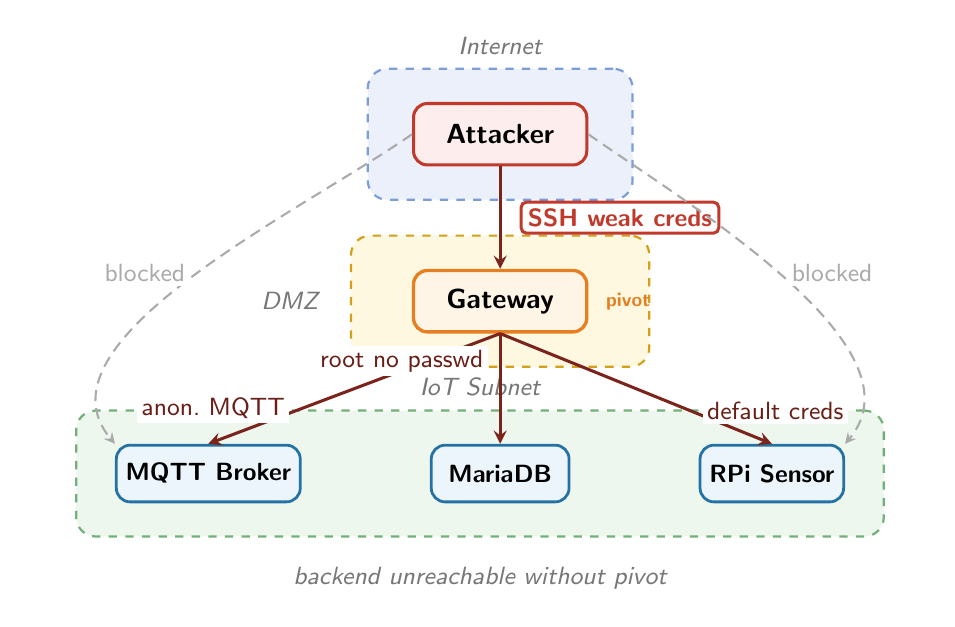
\begin{tikzpicture}[
  natt/.style={draw=AttBorder,fill=AttFill,line width=1.1pt,
    rounded corners=5pt,minimum width=2.2cm,minimum height=0.78cm,
    font=\sffamily\bfseries\normalsize},
  ngw/.style={draw=GwBorder,fill=GwFill,line width=1.2pt,
    rounded corners=5pt,minimum width=2.2cm,minimum height=0.78cm,
    font=\sffamily\bfseries\normalsize},
  nback/.style={draw=BackBorder,fill=BackFill,line width=1.0pt,
    rounded corners=5pt,minimum width=1.75cm,minimum height=0.72cm,
    font=\sffamily\bfseries\small},
  arr/.style={->,>=stealth,draw=FigArrow,line width=1.1pt},
  blk/.style={->,>=stealth,draw=FigBlocked,line width=0.75pt,
    dashed,dash pattern=on 4pt off 2.5pt},
  lbl/.style={font=\sffamily\small,text=FigArrow!85!black,
    fill=white,inner sep=1.5pt,midway},
  badge/.style={draw=AttBorder,fill=white,rounded corners=2pt,
    font=\sffamily\small\bfseries,text=AttBorder,inner sep=2.5pt,midway},
  blbl/.style={font=\sffamily\small,text=FigBlocked,fill=white,
    inner sep=1.5pt,midway},
  zlbl/.style={font=\sffamily\small\itshape,text=FigSubtle}
]
\node[natt] (atk) {Attacker};
\node[ngw, below=1.3cm of atk] (gw) {Gateway};
\node[font=\sffamily\scriptsize\itshape\bfseries,text=GwBorder,
      right=0.1cm of gw.east,anchor=west] {pivot};
\node[nback,below left=1.4cm and 1.4cm of gw]  (mqtt){MQTT Broker};
\node[nback,below=1.4cm of gw]                  (db)  {MariaDB};
\node[nback,below right=1.4cm and 1.4cm of gw]  (rpi) {RPi Sensor};
\begin{scope}[on background layer]
  \node[fill=ZIFill,draw=ZIBorder,dashed,line width=0.8pt,
    rounded corners=7pt,inner xsep=16pt,inner ysep=12pt,fit=(atk)](zI){};
  \node[fill=ZDFill,draw=ZDBorder,dashed,line width=0.8pt,
    rounded corners=7pt,inner xsep=22pt,inner ysep=12pt,fit=(gw)](zD){};
  \node[fill=ZCFill,draw=ZCBorder,dashed,line width=0.8pt,
    rounded corners=7pt,inner xsep=14pt,inner ysep=12pt,
    fit=(mqtt)(db)(rpi)](zC){};
\end{scope}
% Zone labels: centered above each zone
\node[zlbl] at ([yshift=8pt]zI.north) {Internet};
\node[zlbl,anchor=east] at ([xshift=-8pt]zD.west) {DMZ};
\node[zlbl] at ([yshift=8pt]zC.north) {IoT Subnet};
\draw[arr] (atk.south)--(gw.north)   node[badge,right=7pt]{SSH weak creds};
\draw[arr] (gw.south)--(mqtt.north)  node[lbl,left=4pt,pos=0.68]{anon.\ MQTT};
\draw[arr] (gw.south)--(db.north)    node[lbl,left=4pt,pos=0.25]{root no passwd};
\draw[arr] (gw.south)--(rpi.north)   node[lbl,right=4pt,pos=0.70]{default creds};
\draw[blk] (atk.west) to[out=215,in=130,looseness=0.8]
  node[blbl,left=3pt,pos=0.48]{blocked} (mqtt.north west);
\draw[blk] (atk.east) to[out=325,in=50,looseness=0.8]
  node[blbl,right=3pt,pos=0.48]{blocked} (rpi.north east);
% Note below the IoT zone box
\node[zlbl,below=0.25cm of zC,align=center]
  {backend unreachable without pivot};
\end{tikzpicture}%
}
\caption{Conceptual pivot-gated attack surface. This diagram is not Scenario~S3,
which is a flat network. Public held-out S20 and S24--S27 use isolated VLANs;
their deepest fixtures require respectively two and three successive pivots,
and direct-access controls are verified before each run.}
\label{fig:attack-chain}
\end{figure}

% ══════════════════════════════════════════════════════════════════════════
% §4 IoTBench
% ══════════════════════════════════════════════════════════════════════════
\section{\systemname: A Network-Scale Benchmark}
\label{sec:iotbench}

\systemname{} is designed to evaluate network-scale IoT/OT assessment rather than isolated-host exploitation. Scenarios are deployed reproducibly from Ansible playbooks on Proxmox and vulnerabilities are injected idempotently. Flat application workflows, logical prerequisite chains, and enforced network pivots are represented separately. In particular, a scenario receives positive network-pivot depth only when routing or firewall checks demonstrate that the target is unreachable from the original evaluator vantage point. Scenarios mix IoT/OT protocols such as MQTT, Modbus, OPC~UA, BACnet, LoRaWAN, CoAP, SNMP, SSH, HTTP, FTP, and Telnet, with per-vulnerability YAML ground truth recording device, IP, severity, category, structural matching contract, indicators, and verification commands.

\medskip\noindent\textbf{Design goals.}
The benchmark is built around three requirements:
\begin{itemize}[leftmargin=*,nosep]
  \item \textbf{Deployability:} every scenario is generated from Ansible and Proxmox artifacts, so runs can be recreated rather than approximated from static descriptions.
  \item \textbf{Reachability awareness:} firewall rules encode which services are exposed from the entry point and which become reachable only after a gateway or zone transition.
  \item \textbf{Scorable evidence:} the oracle records expected indicators and verification commands, allowing the evaluator to distinguish shallow detection from stronger exploit evidence.
\end{itemize}

The benchmark has 19 public development scenarios and ten inspectable public held-out tests (Table~\ref{tab:scenarios}). Held-out denotes exclusion from empirical tuning, not secrecy.

\begin{table}[h!]
\centering
\caption{\systemname{} scenario catalogue.}
\label{tab:scenarios}
\scriptsize
\setlength{\tabcolsep}{3pt}
\begin{tabular}{@{}llrrr@{}}
\toprule
IDs & Role in protocol & Dev & Vulns & Controls \\
\midrule
\texttt{S1--S12} & Legacy public development and scale & 116 & 209 & 0 \\
\texttt{S13} & VLAN segmentation development fixture & 17 & 20 & 0 \\
\texttt{S14} & Development: mixed-hardening controls & 11 & 4 & 8 \\
\texttt{S15--S18} & Development: logical dependency chains & 28 & 14 & 14 \\
\texttt{S19} & Development: safe OT protocol checks & 8 & 5 & 2 \\
\texttt{S20} & Public held-out: two network pivots & 5 & 4 & 3 \\
\texttt{S21--S22} & Public held-out: prevalence/diversity & 26 & 6 & 22 \\
\texttt{S23} & Public held-out: firmware chain & 9 & 4 & 4 \\
\texttt{S24--S27} & Held-out: enforced network-path stress tests & 28 & 15 & 9 \\
\texttt{S28} & Held-out: provisioning dependency chain & 9 & 4 & 4 \\
\texttt{S29} & Held-out: large sparse-control network & 21 & 3 & 22 \\
\midrule
\textbf{Public total} & & \textbf{278} & \textbf{288} & \textbf{88} \\
\bottomrule
\end{tabular}
\end{table}

\subsection{Deterministic Vulnerability Injection}
\label{sec:iotbench:inject}

Vulnerabilities are injected by a dedicated Ansible role parameterized by \texttt{scenario\_id}, making deployments reproducible and idempotent. Scenario YAML files declare router-level weaknesses (Telnet, WAN administration, FTP) and per-service roles that trigger targeted injections such as anonymous MQTT, weak SSH credentials, and passwordless database roots.

Across both public splits, \systemname{} injects 288 vulnerabilities and evaluates 88 controls. S1--S19 support development and audits. S20--S29 are code-excluded from the learning loop and run only after the harness, prompts, adapters, and budgets are frozen. Their definitions and ground truth remain public for auditability; blind workers receive only the network scope during execution.

\subsection{Ground-Truth Schema}
\label{sec:iotbench:gt}

Each public scenario ships a YAML ground-truth file with one entry per injected vulnerability. Entries record the affected device, IP, role, severity, category, optional CVE, accepted semantic types, structural matching fields, expected indicators, verification command, and two distinct depth variables. \texttt{network\_pivot\_depth} counts enforced changes of network vantage point; \texttt{dependency\_depth} counts ordered logical prerequisites. The historical \texttt{hop\_depth} field is ignored by the v3.4 MHR scorer.

Scenarios may declare tightly bounded advisory types, but these are capped, deduplicated, and require traceable evidence. Hardened comparators are encoded as explicit negative controls and reported separately as a clean-run rate.

\subsection{Scoring and Diagnostic Fields}
\label{sec:iotbench:eval}

Each LLM finding is matched one-to-one to ground truth under a versioned explicit contract. A match requires the target IP, an accepted semantic type (or a target-bound, offline-validated CVE), and the vulnerability-specific \texttt{required\_dimensions}. Optional declared dimensions reject contradictions but are not all mandatory. There is no IP--severity fallback. Unmatched findings are false positives and duplicate claims are collapsed.

The main table reports three values. \emph{Detection F1} measures correctly identified vulnerabilities whether or not exploitation succeeds. \emph{Verified F1}, the primary score, counts a true positive only when a fresh Phase~4 tool record is target-compatible and its output semantically demonstrates the finding. \emph{Verified Severity Coverage} is the fraction of total ground-truth severity weight (critical~4, high~3, medium~2, low~1) whose vulnerabilities are verified. Missing proof in a contract-compatible run receives zero verified credit.

For depth $k$, MHR@k is recall restricted to vulnerabilities with \texttt{network\_pivot\_depth}$\geq k$; DHR@k applies the same definition to \texttt{dependency\_depth}. Verified variants additionally require proof. Undefined depths are reported as N/A rather than zero. Attack-path coverage requires all referenced findings; verified path coverage also requires proof and an ordered Phase~5 chain.

% ══════════════════════════════════════════════════════════════════════════
% §5 Harness
% ══════════════════════════════════════════════════════════════════════════
\section{\harnessname: An LLM Agent for Network Compromise Evaluation}
\label{sec:harness}

Existing LLM pentest harnesses typically process targets as a flat list, letting context grow with network size. \harnessname{} instead decomposes network assessment into six phases with typed deliverables. Its key design choice is device- and vulnerability-level parallelism: constrained micro-agents analyze individual targets or findings, and their outputs are merged deterministically into a network-level state. This keeps early-stage contexts bounded as the number of devices grows, while cross-device reasoning is deferred to the intrusion and reporting phases. LLM-produced vulnerability types are canonicalized into the benchmark taxonomy before scoring, reducing noise and duplicate findings.

\subsection{Pipeline}
\label{sec:harness:pipeline}

\harnessname{} separates network assessment into discovery, local analysis, evidence collection, lateral movement, and reporting. \textbf{Phase~1} builds a directed topology graph $G=(V,E)$ whose vertices are devices and whose edges are protocol-labeled links. In informed mode, this graph is loaded from benchmark metadata; in blind mode, it starts empty and is populated by active discovery. \textbf{Phase~2} scans the target CIDR for hosts, services, versions, L2 vendors, and protocol endpoints (MQTT, SSH, HTTP). \textbf{Phase~3} performs per-device triage: each device receives a deterministic scanner pass and a constrained LLM micro-agent, whose outputs are merged and deduplicated. \textbf{Phase~4} verifies candidate findings with operational tools such as SSH, MQTT, MySQL, Modbus, and Telnet, attempting the deepest evidence level achievable (\textsf{L1}--\textsf{L3}). \textbf{Phase~5} conducts intrusion and lateral movement over observed or asserted topology edges, recording each hop with source, destination, protocol, and credentials. \textbf{Phase~6} emits a network-scoped report with device inventory, validated findings, attack-surface summary, intrusion narrative, and remediation priorities.

\subsection{Cost Envelope}
\label{sec:harness:cost}

For a network with $n$ devices and $v$ candidate findings per device on average, \harnessname{} issues $O(nv)$ LLM invocations: four global calls (Phases~1, 2, 5, and~6), $n$ per-device triage calls (Phase~3), and $nv$ per-finding verification calls (Phase~4). Each invocation has a fixed turn budget (50 for Phases~1--2, 10 for Phases~3--4, 30 for Phase~5, and 20 for Phase~6), so cost scales with observed devices and findings rather than with combinations of network paths.

% ══════════════════════════════════════════════════════════════════════════
% §6 Experimental Setup
% ══════════════════════════════════════════════════════════════════════════
\section{Experimental Setup}
\label{sec:setup}

\textbf{Infrastructure.}
All scenarios run as LXC containers on a Proxmox VE host, connected through a dedicated Linux bridge with an OpenWrt gateway. Deployment and teardown are fully automated with Ansible.

\textbf{Model.}
For the architecture comparison, all LLM-driven systems use the same general-purpose model, \textbf{MiniMax-M2.7}~\cite{minimax27}, with fixed prompts and temperature~0 decoding. This controls for model choice while focusing the comparison on architecture rather than fine-tuning.

\textbf{Baselines.}
We compare \harnessname{} with two adapted LLM-agent baselines:
\begin{itemize}[leftmargin=*,nosep]
  \item a CAI-style single-agent tool loop~\cite{cai25};
  \item a VulnBot-style multi-agent pipeline with a penetration task graph~\cite{vulnbot25}.
\end{itemize}
The confirmatory comparison runs every system in blind mode from the same pre-committed network scope. Baseline adapters must emit the same target, type, structural fields, evidence references, and tool-call provenance as \harnessname{}; the normalizer may not read ground truth or synthesize missing fields. Informed \harnessname{} runs are secondary diagnostics and are not part of the primary architecture comparison.

\textbf{Metrics and variance.}
We report Detection F1, Verified F1 (primary), Verified Severity Coverage, clean-run rate, verified path coverage, verified MHR/DHR, cost, and planned/completed run counts. The confirmatory matrix is \{\harnessname{}, CAI, VulnBot\}$\times$S20--S29$\times$three paired repetitions. Repetitions are averaged within scenario before a ten-scenario macro-average. A pre-committed but missing repetition contributes zero; no incomplete metric is silently omitted. We report paired effect sizes and 95\% confidence intervals across scenario-matched repetitions.

% ══════════════════════════════════════════════════════════════════════════
% §7 Evaluation
% ══════════════════════════════════════════════════════════════════════════
\section{Evaluation}
\label{sec:eval}

\subsection{Pre-registered Confirmatory Matrix}

The primary architecture comparison comprises 90 blind public held-out runs:
three systems (\harnessname{}, CAI, and VulnBot), ten test scenarios
(S20--S29), and three paired repetitions. The campaign manifest fixes the runner
commit, model and provider, tool proxy, budgets, scoring policy, scenario order,
and planned grid before any test run. Harness, prompts,
adapters, and normalizers are then frozen. A missing cell receives zero on all
three scores; completeness is published.

\subsection{Public Diagnostics and Reporting}

S14--S19 receive 36 informed/blind exploratory runs. Before freezing, a 12-run
smoke pilot on S14, S15, and S19 validates infrastructure and adapters but is
excluded from estimates. After the 90 blind runs, S20--S29 receive 30 informed
\harnessname{} runs as a secondary oracle-gap diagnostic. These runs cannot be
used to tune the reported version.

The main result table contains, for each system, Detection F1, Verified F1,
Verified Severity Coverage, clean-run rate, verified path coverage, verified
MHR@1/2/3, cost, and completed/planned runs. We report paired differences against
\harnessname{} with 95\% confidence intervals. Numerical cells are inserted
only after the full pre-committed public test grid has completed. Consequently,
the historical strict-v2 table below is retained
in the source for provenance but deliberately excluded from this draft.

\iffalse

\subsection{Overall Performance}
\label{sec:eval:overall}

Table~\ref{tab:scenario-scores} reports per-scenario F1 across all four systems. Informed \harnessname{} reaches 0.935 mean F1 (0.959 recall, 0.914 precision), while blind \harnessname{} reaches 0.887 mean F1 without a topology prior. Both modes outperform both adapted baselines on every scenario, and the baselines never exceed F1~=~0.55. The scalability scenarios confirm the trend: \texttt{S11} (15 devices) reaches F1~=~0.875 and \texttt{S12} (35 devices) reaches F1~=~0.942 in informed mode.

\begin{table}[h!]
\centering
\caption{\footnotesize Per-scenario F1 on all 12 scenarios (reference run).}
\label{tab:scenario-scores}
\scriptsize
\setlength{\tabcolsep}{3pt}
\begin{tabular}{@{}lrrrr@{}}
\toprule
Scenario & Informed & Blind & CAI & VulnBot \\
\midrule
\texttt{S1}  & 0.923 & 0.880 & 0.153 & 0.153 \\
\texttt{S2}  & 0.923 & 0.923 & 0.353 & 0.445 \\
\texttt{S3}  & 0.947 & 0.941 & 0.000 & 0.000 \\
\texttt{S4}  & 0.944 & 0.909 & 0.363 & 0.435 \\
\texttt{S5}  & 1.000 & 0.929 & 0.500 & 0.500 \\
\texttt{S6}  & 1.000 & 1.000 & 0.400 & 0.400 \\
\texttt{S7}  & 0.965 & 0.889 & 0.500 & 0.445 \\
\texttt{S8}  & 0.933 & 0.923 & 0.546 & 0.353 \\
\texttt{S9}  & 0.952 & 0.857 & 0.167 & 0.286 \\
\texttt{S10} & 0.815 & 0.769 & 0.143 & 0.143 \\
\texttt{S11} & 0.875 & 0.857 & 0.414 & 0.414 \\
\texttt{S12} & 0.942 & 0.762 & 0.242 & 0.307 \\
\midrule
Mean         & 0.935 & 0.887 & 0.315 & 0.323 \\
\bottomrule
\end{tabular}
\smallskip\\
\footnotesize\emph{F1~=~0 means that the normalized output contained no finding matching the scenario ground truth under the common evaluator.}
\end{table}

Beyond F1, informed \harnessname{} reaches 86.4\% severity-weighted score on average, compared with 73.8\% in blind mode. Blind mode has slightly higher mean precision (0.922 vs.\ 0.914) but lower recall (0.856 vs.\ 0.959), showing that active discovery reduces some false positives while missing vulnerabilities that the topology prior helps expose or prioritize. The clearest multi-hop failure case is \texttt{S3}: both adapted baselines produce no true-positive matches, while \harnessname{} remains above F1~=~0.94 in both modes.

\textbf{Per-scenario interpretation.}
The scenario spread helps explain the aggregate result. \texttt{S3} isolates pivot reasoning: the vulnerable back-end services are present but unreachable until the gateway is traversed, so flat per-target baselines fail even when run with target knowledge. \texttt{S10} is the lowest informed \harnessname{} score (F1~=~0.815), indicating that role variants and naming heterogeneity still create matching and prioritization errors. \texttt{S12} stresses network size: informed \harnessname{} remains high on 35 devices (F1~=~0.942), while blind mode drops to 0.762, showing that active discovery remains useful but topology metadata becomes more valuable as the device set grows. These cases motivate reporting per-scenario scores rather than only macro averages.

\subsection{Rerun Consistency}
\label{sec:eval:consistency}

To estimate run-to-run stability, informed \harnessname{} was executed twice on the same artifact set. The second run reaches mean F1~=~0.918 versus 0.935 for the reference run ($\Delta=-0.017$). Seven scenarios vary by less than 0.05 F1; the largest drops occur on \texttt{S7} ($-0.182$) and \texttt{S4} ($-0.156$), while \texttt{S10} improves by $+0.145$. Blind mode was executed once per scenario, so full blind-mode confidence intervals remain future work.

\subsection{Model Sensitivity}
\label{sec:eval:model-sensitivity}

To assess whether \harnessname{} depends on a single LLM backend, we rerun the same architecture with MiniMax-M2.7, DeepSeek V4 Flash, Gemma 4 12B, and Qwen3-14B under identical prompts, tool budgets, artifacts, and evaluator. Table~\ref{tab:model-sensitivity} reports macro-averaged results over the same 12 scenarios. The three additional backends remain close to the MiniMax reference: F1 ranges from 0.945 to 0.947, while severity-weighted score ranges from 83.0\% to 85.5\%.

\begin{table}[h!]
\centering
\caption{\footnotesize Model sensitivity of \harnessname{} on \systemname{}.}
\label{tab:model-sensitivity}
\scriptsize
\setlength{\tabcolsep}{4pt}
\begin{tabular}{@{}lrrrr@{}}
\toprule
Model & Recall & Precision & F1 & Sev.-weighted \\
\midrule
MiniMax-M2.7       & 0.959 & 0.914 & 0.935 & 86.4\% \\
DeepSeek V4 Flash  & 0.933 & 0.964 & 0.947 & 85.5\% \\
Gemma 4 12B        & 0.917 & 0.976 & 0.945 & 83.0\% \\
Qwen3-14B          & 0.923 & 0.976 & 0.947 & 84.1\% \\
\bottomrule
\end{tabular}
\end{table}

The main cross-model variation is a precision--recall tradeoff rather than a collapse in task performance: Gemma and Qwen are more conservative, while DeepSeek obtains the highest severity-weighted score among the additional backends.

\subsection{Single-Host Transfer Checks}
\label{sec:eval:transfer}

Although the main claim concerns network-scale IoT evaluation, we also run \harnessname{} on two established single-host corpora to check that the per-target exploitation component is not specialized only to \systemname{}. These runs are contextual rather than a controlled leaderboard because task oracles and published protocols differ across systems. On AutoPenBench, informed \harnessname{} captures 9/33 end-to-end flags (27.3\%) and produces useful exploit evidence on 17/33 tasks (51.5\%); blind mode captures 7/33 flags (21.2\%). On a 328-case Vulhub snapshot, informed \harnessname{} produces 99 useful findings (30.2\%), while blind mode produces 92 (28.0\%). These results support transfer to single-host exploitation, but they do not replace the main \systemname{} result because they do not exercise topology priors, reachability constraints, or lateral movement.

\fi

% ══════════════════════════════════════════════════════════════════════════
% §8 Discussion
% ══════════════════════════════════════════════════════════════════════════
\section{Discussion and Limitations}
\label{sec:discussion}

The revised design isolates three questions that the previous evaluation mixed.
\begin{itemize}[leftmargin=*,nosep]
  \item \textbf{Identification is not verification.} Detection F1 measures whether the system names the right vulnerability; Verified F1 determines whether the claim is supported by fresh target-bound execution evidence.
  \item \textbf{Logical depth is not network depth.} S15--S18, S23, and S28 test ordered application prerequisites through DHR. Only infrastructure-enforced reachability transitions, such as S20 and S24--S27, contribute to MHR.
  \item \textbf{Controls are not positive findings.} Hardened comparators produce a separate clean-run rate. Mixing them into a composite F1 obscures whether a failure comes from missed vulnerabilities or over-reporting.
\end{itemize}

Several limitations remain.
\begin{itemize}[leftmargin=*,nosep]
  \item \textbf{Virtualization boundary:} scenarios run on Linux containers; real constrained hardware, bootloaders, RTOS firmware, and physical interfaces introduce attack surfaces not covered here.
  \item \textbf{Public hold-out contamination:} auditability makes S20--S29 inspectable. The protection is procedural---pre-commitment, blind execution, and a prohibition on tuning from test results---rather than secrecy; future repeated development requires a new test edition.
  \item \textbf{Oracle boundaries:} matching contracts and bounded advisory categories still require expert review even though severity fallback has been removed.
  \item \textbf{Prompt and model scope:} results use a single prompt family; per-model prompt tuning may change absolute scores even if the architecture trend persists.
  \item \textbf{Scenario coverage:} the benchmark covers fixed topological patterns and vulnerabilities tractably injectable via Ansible; dynamic deployments, RF-layer attacks, and supply-chain weaknesses are out of scope.
\end{itemize}

% ══════════════════════════════════════════════════════════════════════════
% §9 Conclusion
% ══════════════════════════════════════════════════════════════════════════
\section{Conclusion}
\label{sec:conclusion}

Single-host benchmarks miss IoT/OT reachability dependencies. We introduce \systemname{}, with 19 public development and ten public held-out scenarios, and \harnessname{}, a six-phase network-native assessment harness.

The methodological contribution is a fail-closed separation of detection,
verified exploitation, severity-weighted coverage, negative controls, logical
dependencies, and enforced network pivots. The final empirical claim will be
drawn only from the pre-committed 90-run blind public-test matrix; development
and informed diagnostic runs are reported separately. We release the scenarios,
playbooks, ground truth, matching contracts, and evaluation code to support
reproducible research in this setting.
% ── bibliography ──────────────────────────────────────────────────────────
\begin{thebibliography}{00}

\bibitem{happe23} A.~Happe and J.~Cito, ``Getting pwn'd by AI: Penetration testing with large language models,'' in \textit{Proc. ACM ESEC/FSE}, 2023.

\bibitem{pentestgpt24} G.~Deng, Y.~Liu, V.~Mayoral-Vilches, P.~Liu, Y.~Li, Y.~Xu, T.~Zhang, Y.~Liu, M.~Pinzger, and S.~Rass, ``PentestGPT: Evaluating and harnessing large language models for automated penetration testing,'' in \textit{Proc. 33rd USENIX Security Symp. (USENIX Security 24)}, 2024, pp.~847--864. [Online]. Available: \url{https://www.usenix.org/conference/usenixsecurity24/presentation/deng}

\bibitem{hackingbuddygpt} A.~Happe \textit{et al.}, ``HackingBuddyGPT: An LLM-driven pentest agent,'' 2024. [Online]. Available: \url{https://github.com/ipa-lab/hackingBuddyGPT}

\bibitem{autoattacker24} J.~Xu \textit{et al.}, ``AutoAttacker: A large language model guided system to implement automatic cyber-attacks,'' \textit{arXiv:2403.01038}, 2024.

\bibitem{vulnbot25} H.~Kong \textit{et al.}, ``VulnBot: Autonomous penetration testing for a multi-agent collaborative framework,'' \textit{arXiv:2501.13411}, 2025. [Online]. Available: \url{https://arxiv.org/abs/2501.13411}

\bibitem{autopentester25} Y.~Ginige \textit{et al.}, ``AutoPentester: An LLM agent-based framework for automated pentesting,'' \textit{arXiv:2510.05605}, 2025.

\bibitem{cai25} V.~Mayoral-Vilches \textit{et al.}, ``CAI: An open, bug bounty-ready cybersecurity AI,'' \textit{arXiv:2504.06017}, 2025.

\bibitem{xoffense25} P.~D.~Luong \textit{et al.}, ``xOffense: An autonomous multi-agent framework for penetration testing with domain-adapted large language models,'' \textit{arXiv:2509.13021}, 2025.

\bibitem{autopenbench24} L.~Gioacchini, M.~Mellia, I.~Drago, A.~Delsanto, G.~Siracusano, and R.~Bifulco, ``AutoPenBench: Benchmarking generative agents for penetration testing,'' \textit{arXiv:2410.03225}, 2024.

\bibitem{vulhub} Vulhub contributors, ``Vulhub: Pre-built vulnerable Docker environments for learning and reproducing CVEs.'' [Online]. Available: \url{https://github.com/vulhub/vulhub}

\bibitem{caibench25} M.~Sanz-G{\'o}mez, V.~Mayoral-Vilches, F.~Balassone, L.~J.~Navarrete-Lozano, C.~R.~J.~Veas Chavez, and M.~del Mundo de Torres, ``Cybersecurity AI Benchmark (CAIBench): A meta-benchmark for evaluating cybersecurity AI agents,'' \textit{arXiv:2510.24317}, 2025. [Online]. Available: \url{https://arxiv.org/abs/2510.24317}

\bibitem{nyuctfbench24} M.~Shao \textit{et al.}, ``NYU CTF Bench: A scalable open-source benchmark dataset for evaluating LLMs in offensive security,'' in \textit{Proc. NeurIPS Datasets and Benchmarks Track}, 2024.

\bibitem{cybench24} A.~K.~Zhang \textit{et al.}, ``Cybench: A framework for evaluating cybersecurity capabilities and risk of language models,'' \textit{arXiv:2408.08926}, 2024.

\bibitem{ludus} Ludus Cloud, ``Ludus: Cyber range automation on Proxmox.'' [Online]. Available: \url{https://ludus.cloud}

\bibitem{goad} M3, ``GOAD: Game of Active Directory.'' [Online]. Available: \url{https://github.com/Orange-Cyberdefense/GOAD}

\bibitem{phillips98} C.~Phillips and L.~P.~Swiler, ``A graph-based system for network-vulnerability analysis,'' in \textit{Proc. New Security Paradigms Workshop}, 1998.

\bibitem{sheyner02} O.~Sheyner, J.~Haines, S.~Jha, R.~Lippmann, and J.~M.~Wing, ``Automated generation and analysis of attack graphs,'' in \textit{Proc. IEEE Symp. Security and Privacy}, 2002.

\bibitem{mulval05} X.~Ou, S.~Govindavajhala, and A.~W.~Appel, ``MulVAL: A logic-based network security analyzer,'' in \textit{Proc. 14th USENIX Security Symp. (USENIX Security 05)}, 2005, pp.~113--128. [Online]. Available: \url{https://www.usenix.org/legacy/events/sec05/tech/full_papers/ou/ou.pdf}

\bibitem{owasp-iot} OWASP Foundation, ``OWASP Internet of Things,'' 2024. [Online]. Available: \url{https://owasp.org/www-project-internet-of-things/}

\bibitem{mitre-ics} MITRE Corporation, ``MITRE ATT\&CK for ICS,'' 2024. [Online]. Available: \url{https://attack.mitre.org/matrices/ics/}

\bibitem{nist80082} K.~Stouffer \textit{et al.}, ``Guide to operational technology security,'' National Institute of Standards and Technology, NIST SP\,800-82 Rev.\,3, 2023.

\bibitem{iot23} S.~Garcia, A.~Parmisano, and M.~J.~Erquiaga, ``IoT-23: A labeled dataset with malicious and benign IoT network traffic,'' Stratosphere Laboratory, 2020. [Online]. Available: \url{https://www.stratosphereips.org/datasets-iot23}

\bibitem{toniot20} A.~Alsaedi, N.~Moustafa, Z.~Tari, A.~Mahmood, and A.~Anwar, ``TON\_IoT telemetry dataset: A new generation dataset of IoT and IIoT for data-driven intrusion detection systems,'' \textit{IEEE Access}, vol.~8, pp.~165130--165150, 2020.

\bibitem{edgeiiotset22} M.~A.~Ferrag, O.~Friha, D.~Hamouda, L.~Maglaras, and H.~Janicke, ``Edge-IIoTset: A new comprehensive realistic cyber security dataset of IoT and IIoT applications for centralized and federated learning,'' \textit{IEEE Access}, vol.~10, pp.~40281--40306, 2022.

\bibitem{costin14} A.~Costin, J.~Zaddach, A.~Francillon, and D.~Balzarotti, ``A large-scale analysis of the security of embedded firmwares,'' in \textit{Proc. 23rd USENIX Security Symp. (USENIX Security 14)}, 2014, pp.~95--110. [Online]. Available: \url{https://www.usenix.org/conference/usenixsecurity14/technical-sessions/presentation/costin}

\bibitem{firmadyne16} D.~D.~Chen, M.~Egele, M.~Woo, and D.~Brumley, ``Towards automated dynamic analysis for Linux-based embedded firmware,'' in \textit{Proc. NDSS}, 2016.

\bibitem{firmae20} M.~Kim, D.~Kim, E.~Kim, S.~Kim, Y.~Jang, and Y.~Kim, ``FirmAE: Towards large-scale emulation of IoT firmware for dynamic analysis,'' in \textit{Proc. Annual Computer Security Applications Conf. (ACSAC)}, 2020.

\bibitem{iotgoat} OWASP, ``IoTGoat: A deliberately insecure IoT firmware,'' 2024. [Online]. Available: \url{https://github.com/OWASP/IoTGoat}

\bibitem{minimax27} MiniMax, ``MiniMax-M2.7: A general-purpose large language model,'' 2026. [Online]. Available: \url{https://www.minimax.io/models/text/m27}

\end{thebibliography}

\end{document}
